\section{Minimal number of measurements}

From now on we will consider only random matrices with $\mathcal{N}(0,1)$-distributed entries.
It might seem unnatural at first if we think of compressive sensing only in the context of natural phenomena.
However, if we look instead at data compression, then we are free to choose the matrix $\A$ however we like.
Considering the vast number of results for normally distributed matrices and normal distribution in general,
they become convenient candidates for the task.

Before proceeding to recovery criteria for random matrices, we first have to recall some definitions from convex geometry.

\begin{definition}
    A convex set $\mathcal{C} \subset \mathbb{R}^N$ is called a \textit{cone} if it is closed under non-negative scalar multiplications, i.e.
    $\forall \alpha \geq 0, \x \in \mathcal{C}: \alpha \x \in \mathcal{C}$.

    The cone $\mathcal{C}^* = \{ \x \in \mathbb{R}^N : \left< \x, \y \right> \leq 0, \ \forall \y \in \mathcal{C} \}$
    is called the \textit{polar} of $\mathcal{C}$.
\end{definition}

\begin{definition}
    Let $C \subset \mathbb{R}^N$ be a convex set and $\x \in \mathbb{R}^N$.
    We call a \textit{tangent cone} of $C$ the cone $T_C(\x) = \op{cl}\{\alpha\x: \x \in C, \alpha \geq 0  \} $.
    We call a \textit{normal cone} of $C$ the cone $N_C(\x) = T_C^*(\x)$.
\end{definition}

\begin{definition}
    The \textit{descent cone} $\mathcal{D}(f, \x) $ of a proper convex function $f: \mathbb{R}^N \rightarrow \overline{\mathbb{R}}$
    at $\x \in \mathbb{R}^N$ is defined as $$\mathcal{D}(f, \x) = \bigcup_{\tau > 0} \left\{ \z \in \mathbb{R}^N: f(\x+\tau \z) \leq f(\x) \right\}. $$
\end{definition}

\begin{remark}
    Tangent cone to level sets
\end{remark}

\begin{proposition}
    The vector $\x \in \mathbb{R}^N$ is the unique solution of \ref{eq:l1} iff $\mathcal{D}(\norm{\cdot}_1, \x) \cap \op{Ker} \A = \{\mathbf{0}\}$.
    \label{th:ker}
\end{proposition}

\begin{proof}
    $(\Leftarrow)$ Let $\x \in \mathbb{R}^N$ and $\mathcal{D}(\norm{\cdot}_1, \x) \cap \op{Ker} \A = \{\mathbf{0}\}$.
    Additionally, we assume that vector $\x$ satisfies linear constraints $\A\x=\y$.
    Suppose that there exists $\z \in \mathbb{R}^N$, $\z \neq \x$, such that $\A\z=\y$ and $\norm{z}_1 \leq \norm{x}_1$.
    Then $\A(\z-\x)=0$ and $z-x \in \op{Ker} \A$.
    By definition, $\mathcal{D}(f, \x) = \bigcup_{\tau > 0} \left\{ \z \in \mathbb{R}^N: \norm{\x+\tau \z}_1 \leq \norm{\x} \right\}$.
    So, $\z - \x \in \mathcal{D}(\norm{\cdot}_1, \x)$ (with $\tau = 1$ we have $\norm{\x + (\z - \x)}_1 \leq \norm{\x}_1$).
    But then $\mathcal{D}(\norm{\cdot}_1, \x) \cap \op{Ker} \A \neq \{\mathbf{0}\}$, which contradicts the hypothesis.
    Thus, $\x$ is the unique minimizer of~\ref{eq:l1}.

    $(\Rightarrow)$ Let $\x \in \mathbb{R}^N$ be the unique solution of~\ref{eq:l1}, i.e, $\x$ satisfies $\A\x=\y$ and
    for any $\x' \neq \x$ such that $\A \x' = \y$, $\norm{\x'}_1 > \norm{\x}_1$.
    Let $\z \in \mathcal{D}(\norm{\cdot}_1, \x)$ and $\z \neq \mathbf{0}$.
    Then there exists $\tau > 0$ such that $\norm{\x + \tau \z}_1 \leq \norm{\x}_1 $.
    If we suppose that $\z \in \op{Ker} \A$, then $\A \z = \mathbf{0}$ and $\A(\x + \tau \z) = \y$.
    As $\x$ is the unique minimizer, it has to be that $\norm{\x + \tau \z}_1 > \norm{\x}_1$, which leads to a contradiction.
    Thus, $\mathcal{D}(\norm{\cdot}_1, \x) \cap \op{Ker} \A = \{\mathbf{0}\}$.
\end{proof}

\begin{figure}
    \begin{subfigure}{0.45\textwidth}
        \begin{tikzpicture}
            \path [fill=teal, fill opacity=0.15] (0, 2) -- (-3.5, -1.5) to[curve through={(-2.5, -2.6) .. (-1.8, -2.7) .. (0, -3.4) ..
            (1.3, -2.9) .. (2, -2.8)}] (3.5, -1.5) -- (0, 2) --cycle;
            \draw [gray, densely dashed][->] (-3.5,0)--(3.5,0);
            \draw [gray, densely dashed][->] (0,-2.2)--(0,3);
            \draw [gray, densely dashed] (0, -3.5) -- (0, -2.8)
            \draw [teal, draw opacity=0.5] (0, 2) -- (-3.5, -1.5);
            \draw [teal, draw opacity=0.5] (0, 2) -- (3.5, -1.5);
            \draw [teal, line width=1pt][shorten <=-3cm] (0,2)--(3.5, 1) node [sloped, pos=0.7, above=-0.1cm] {$\op{Ker}\A+\x^*$};
            \draw [pattern=vertical lines, fill opacity=0.25](-2,0)--(0,2)--(2,0)--(0,-2)--cycle;
            \draw[black] [-{Circle[width=3pt, length=3pt, fill=black, black]}, shorten >=-1.5pt] (0,2) node [above right] {$\x^*$};
            \node at (0, -2.5) {$\mathcal{D}(\norm{\cdot}_1, \x^*)+\x^*$};
        \end{tikzpicture}
        \caption{}
    \end{subfigure}
    \hfill
    \begin{subfigure}{0.45\textwidth}
        \begin{tikzpicture}
            \path [fill=teal, fill opacity=0.15] (0, 2) -- (-3.5, -1.5) to[curve through={(-2.5, -2.6) .. (-1.8, -2.7) .. (0, -3.4) ..
            (1.3, -2.9) .. (2, -2.8)}] (3.5, -1.5) -- (0, 2) --cycle;
            \draw [gray, densely dashed][->] (-3.5,0)--(3.5,0);
            \draw [gray, densely dashed][->] (0,-2.2)--(0,3);
            \draw [gray, densely dashed] (0, -3.5) -- (0, -2.8)
            \draw [teal, draw opacity=0.5] (0, 2) -- (-3.5, -1.5);
            \draw [teal, draw opacity=0.5] (0, 2) -- (3.5, -1.5);
            \draw [teal, line width=1pt][shorten <=-1cm] (0,2)--(2.5, -3.5) node [pos=0, above left=0.3cm] {$\op{Ker}\A+\x^*$};
            \draw [pattern=vertical lines, fill opacity=0.25](-2,0)--(0,2)--(2,0)--(0,-2)--cycle;
            \draw[black] [-{Circle[width=3pt, length=3pt, fill=black, black]}, shorten >=-1.5pt] (0,2) node [above right] {$\x^*$};
            \node at (0, -2.5) {$\mathcal{D}(\norm{\cdot}_1, \x^*)+\x^*$};
        \end{tikzpicture}
        \caption{}
    \end{subfigure}
    \caption{descent cone}
    \label{fig:desc_cone}
\end{figure}

\subsection{Gaussian width approach}

\begin{figure}
    \begin{subfigure}{0.5\linewidth}
        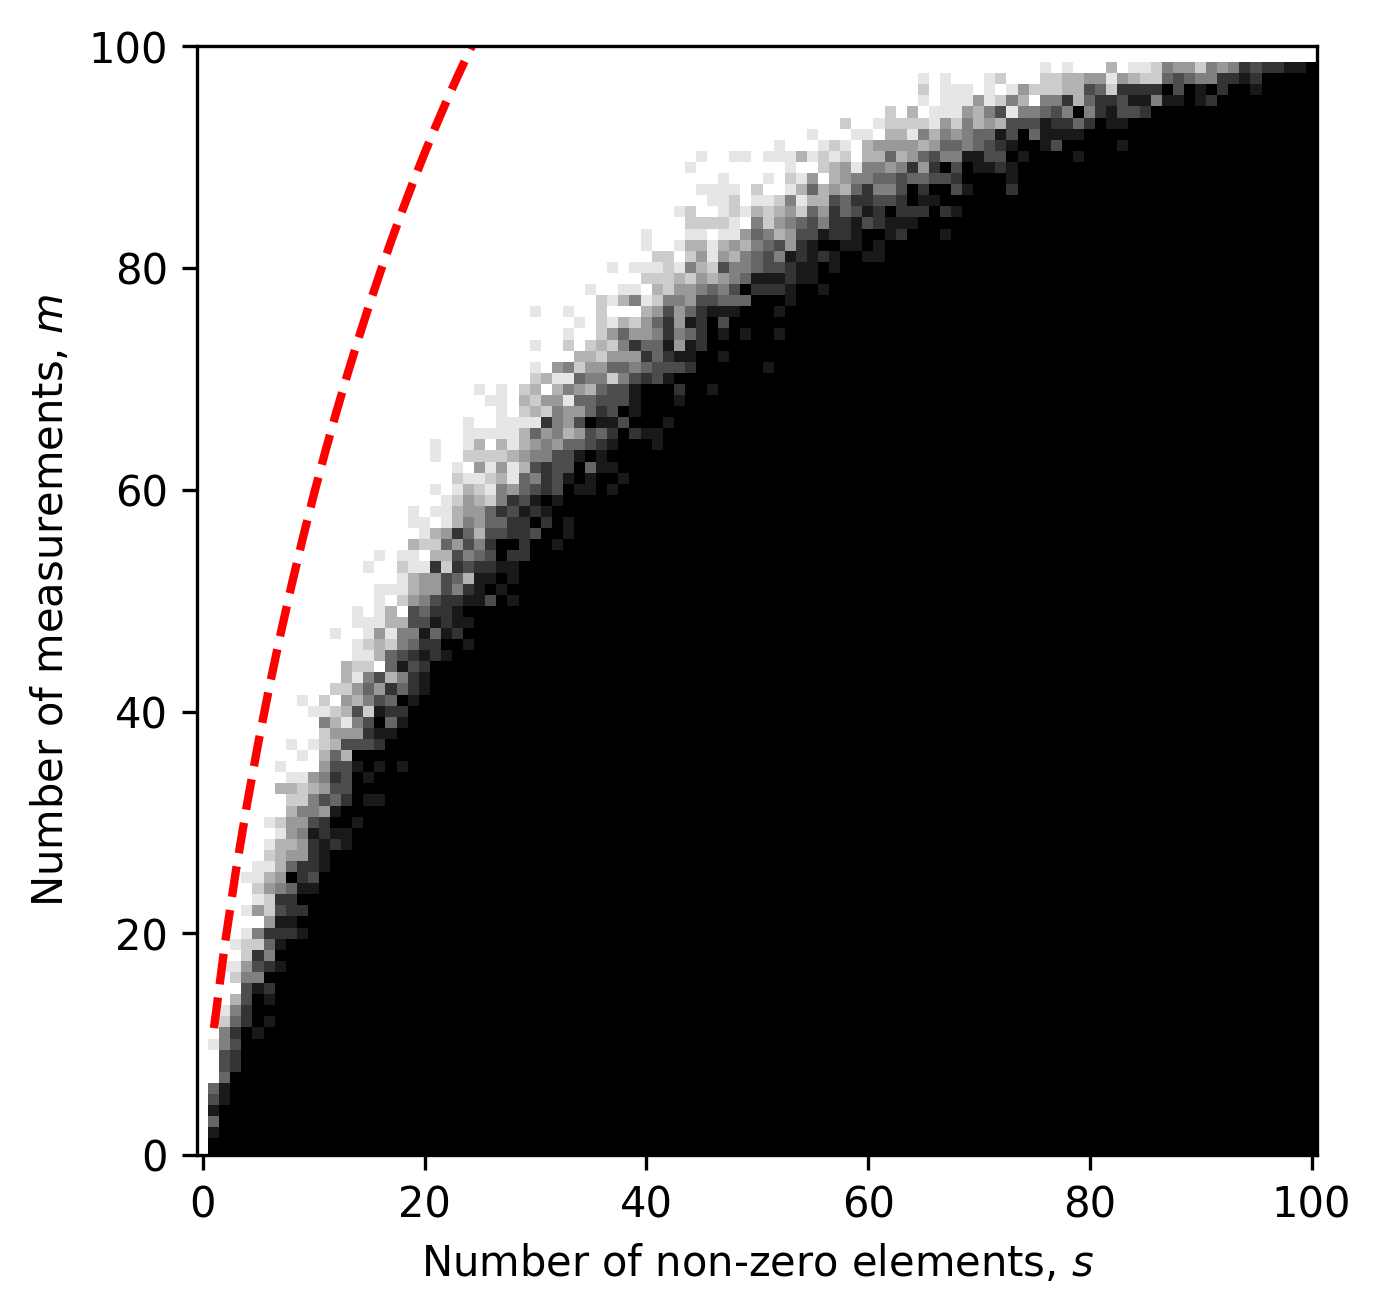
\includegraphics[width=\linewidth]{pictures/log_estimate.png}
        \caption{}
    \end{subfigure}
    \begin{subfigure}{0.5\linewidth}
        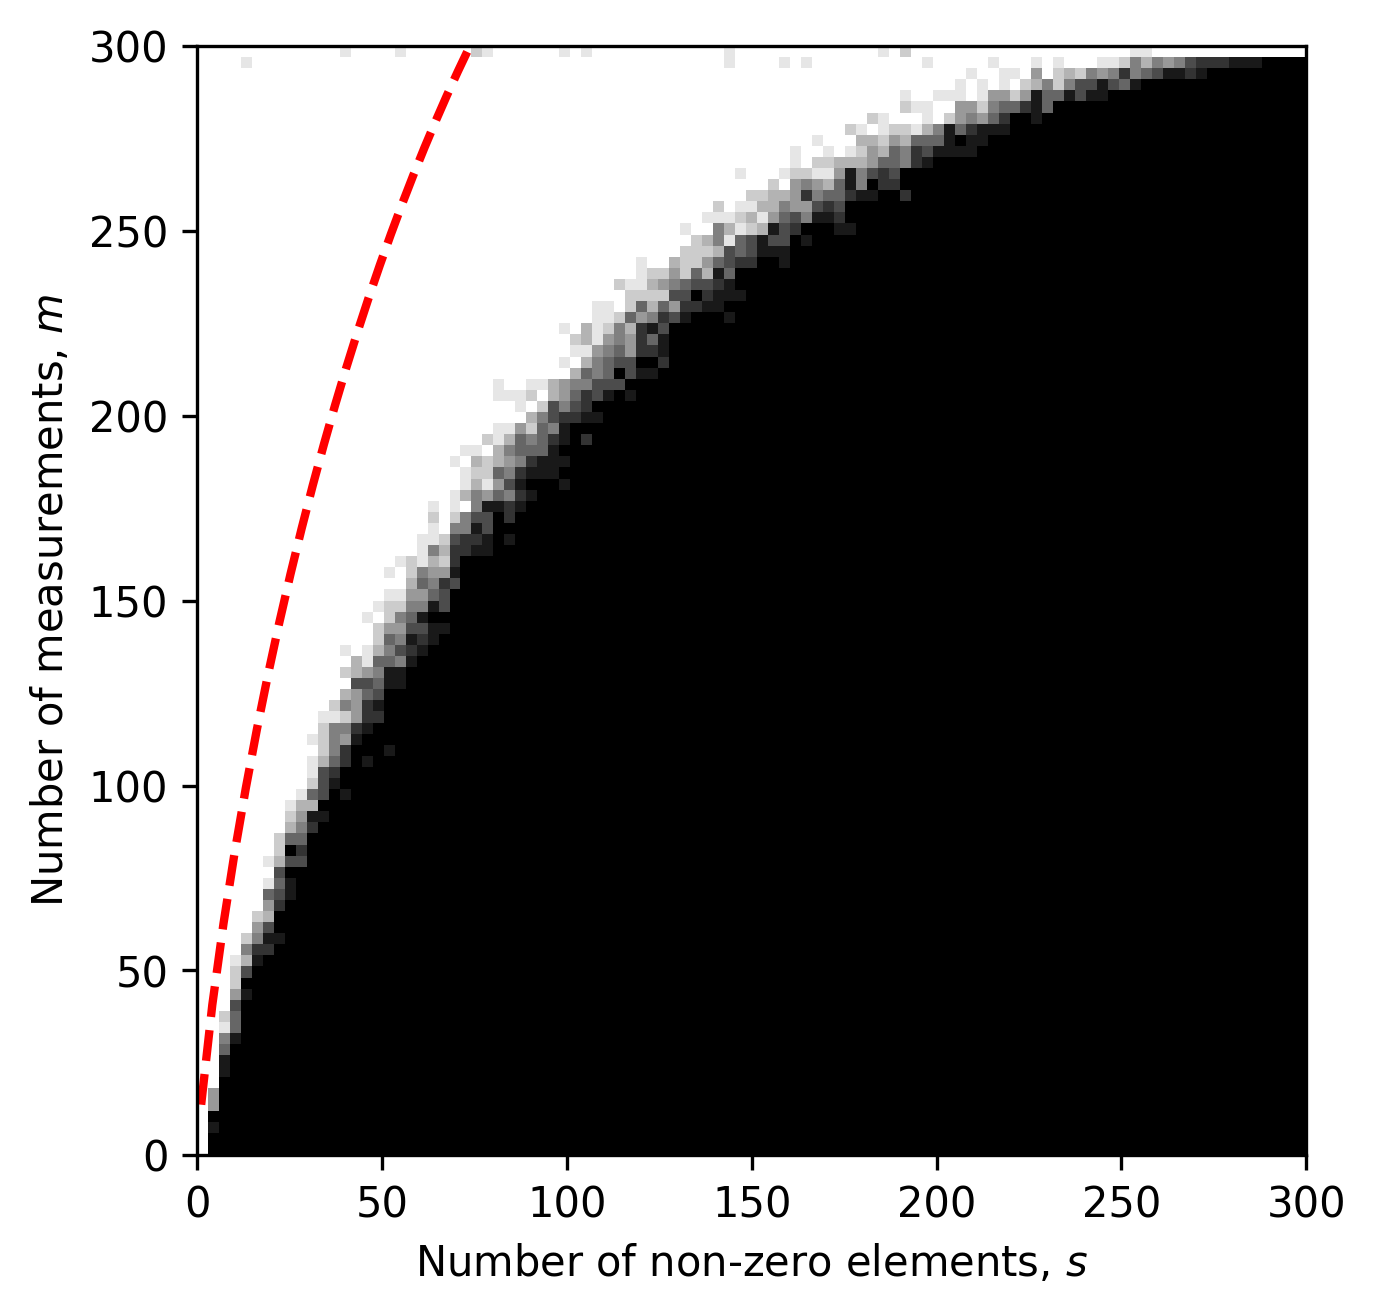
\includegraphics[width=\linewidth]{pictures/log_estimate300.png}
        \caption{}
    \end{subfigure}
    \caption{}
    \label{fig:log}
\end{figure}

\begin{definition}
    Let $\mathcal{A} \subset \mathbb{R}^{N}$ be a compact set of atoms.
    The atomic norm of $\x \in \mathbb{R}^N$ is then defined as
    \[ \norm{\x}_\mathcal{A} = \inf \left\{  \sum_{\mathbf{a} \in \mathcal{A}}c_\mathbf{a}:
                                        \x = \sum_{\mathbf{a} \in \mathcal{A}}c_\mathbf{a} \mathbf{a},
        ~c_\mathbf{a} \geq 0 \ \forall\mathbf{a} \in \mathcal{A} \right\}. \]
\end{definition}

We are interested only in the specific case of the $l_1$ norm which can be interpreted as an atomic norm with
$\mathcal{A} = \cup_{k=1}^N \{ \mathbf{e}^{(k)}: e^{(k)}_k = 1, e^{(k)}_j = 0 \ \forall j \neq k \}$, i.e., the standard basis.

\begin{definition}
    The \textit{Gaussian width} of a set $S \subset \mathbb{R}^N$ is defined as
    \[ w(S) = \mathbb{E} \left[ \sup_{\z \in S} \mathbf{g}^T \z \right], \]
    where $\mathbf{g} \sim \mathcal{N}(\mathbf{0}, \mathbf{I})$ is a vector of i.i.d. random variables with standard normal distribution.
\end{definition}

\begin{theorem}\label{th:yibucha}
    Let $\A \in M_{m \times N}$ be a random matrix with i.i.d components with $\mathcal{N}(0, 1)$ distribution,
    $\x^* \in \mathbb{R}^N$ and let $\Omega = T_{\mathcal{A}}(\x^*) \cap \mathbb{S}^{N-1}$.
    Suppose that $\y = \A \x^*$.
    Then
    \[ m \geq w(\Omega)^2 + 1 \implies \mathbb{P}\{ \x^* \text{ is the unique solution of \ref{eq:l1}} \} \geq
    1-\exp\left(-\frac{1}{2}(\lambda_m - w(\Omega))^2\right),\]
    where $\lambda_m$ is the expected length of an $m$-dimensional gaussian vector.
\end{theorem}

\begin{proposition}
    Let $\x^* \in \mathbb{R}^N$ be an $s$-sparse vector.
    We have the following inequality:
    \[ w(T_{\mathcal{A}}(\x^*)\cap \mathbb{S}^{N-1})^2 \leq 2s \log \frac{N}{s} + \frac{5}{4}s.\]
\end{proposition}
If we combine this result with Theorem~\ref{th:yibucha}, we get the following condition for successful recovery:
\begin{align}
     m \geq 2s\log \frac{N}{s} + \frac{5}{4}s + 1 \implies &\mathbb{P}\{\x^* \text{ is the unique solution of \ref{eq:l1}}\} \nonumber \\
    & \geq 1 - \exp \left( - \frac{1}{2} \left[\lambda_m - w(\Omega)\right]^2 \right) \label{eq:log}.
\end{align}
In Fig.~\ref{fig:log} we can see this estimate applied to dimensions 100 and 300.

\begin{figure}
    \begin{subfigure}{0.5\textwidth}
        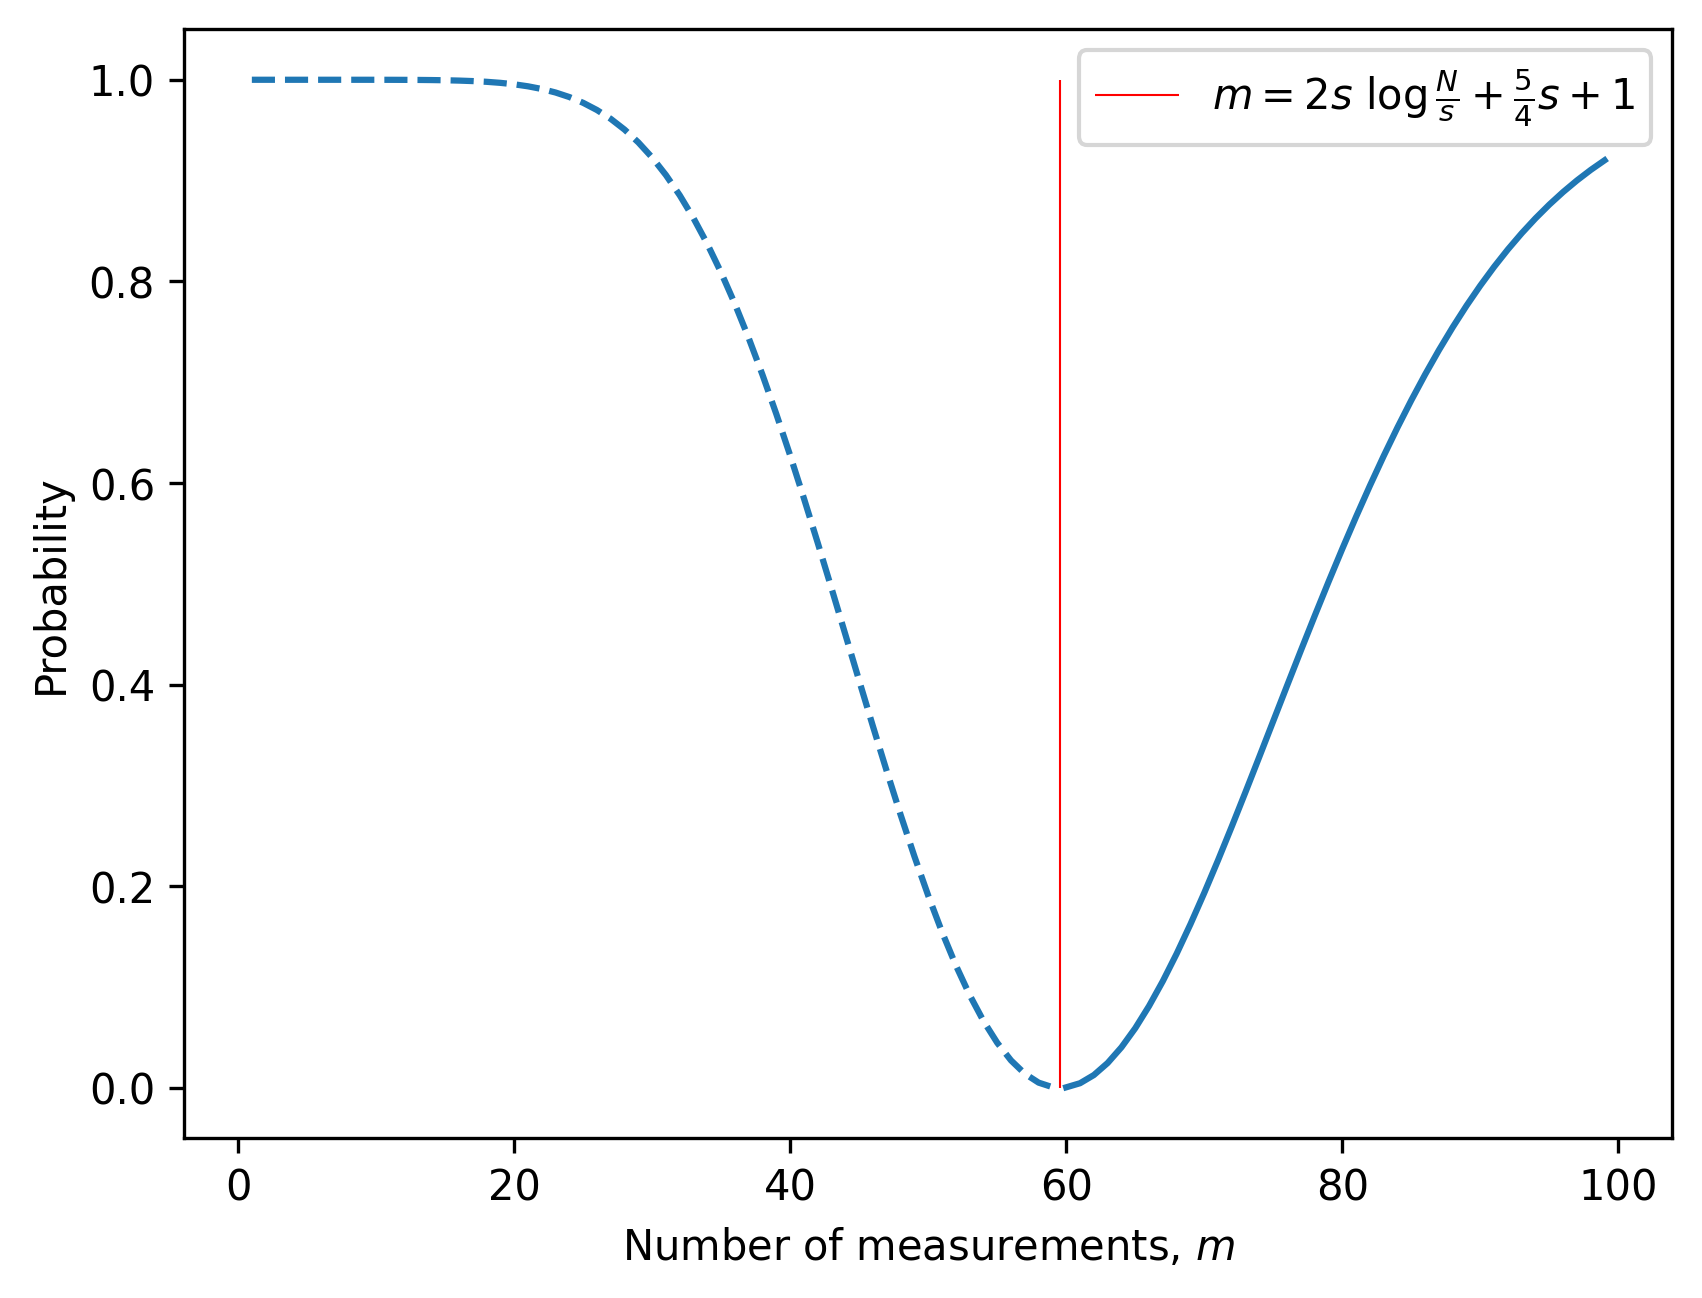
\includegraphics[width=\linewidth]{pictures/log_proba100}
        \caption{}
    \end{subfigure}
    \begin{subfigure}{0.5\textwidth}
        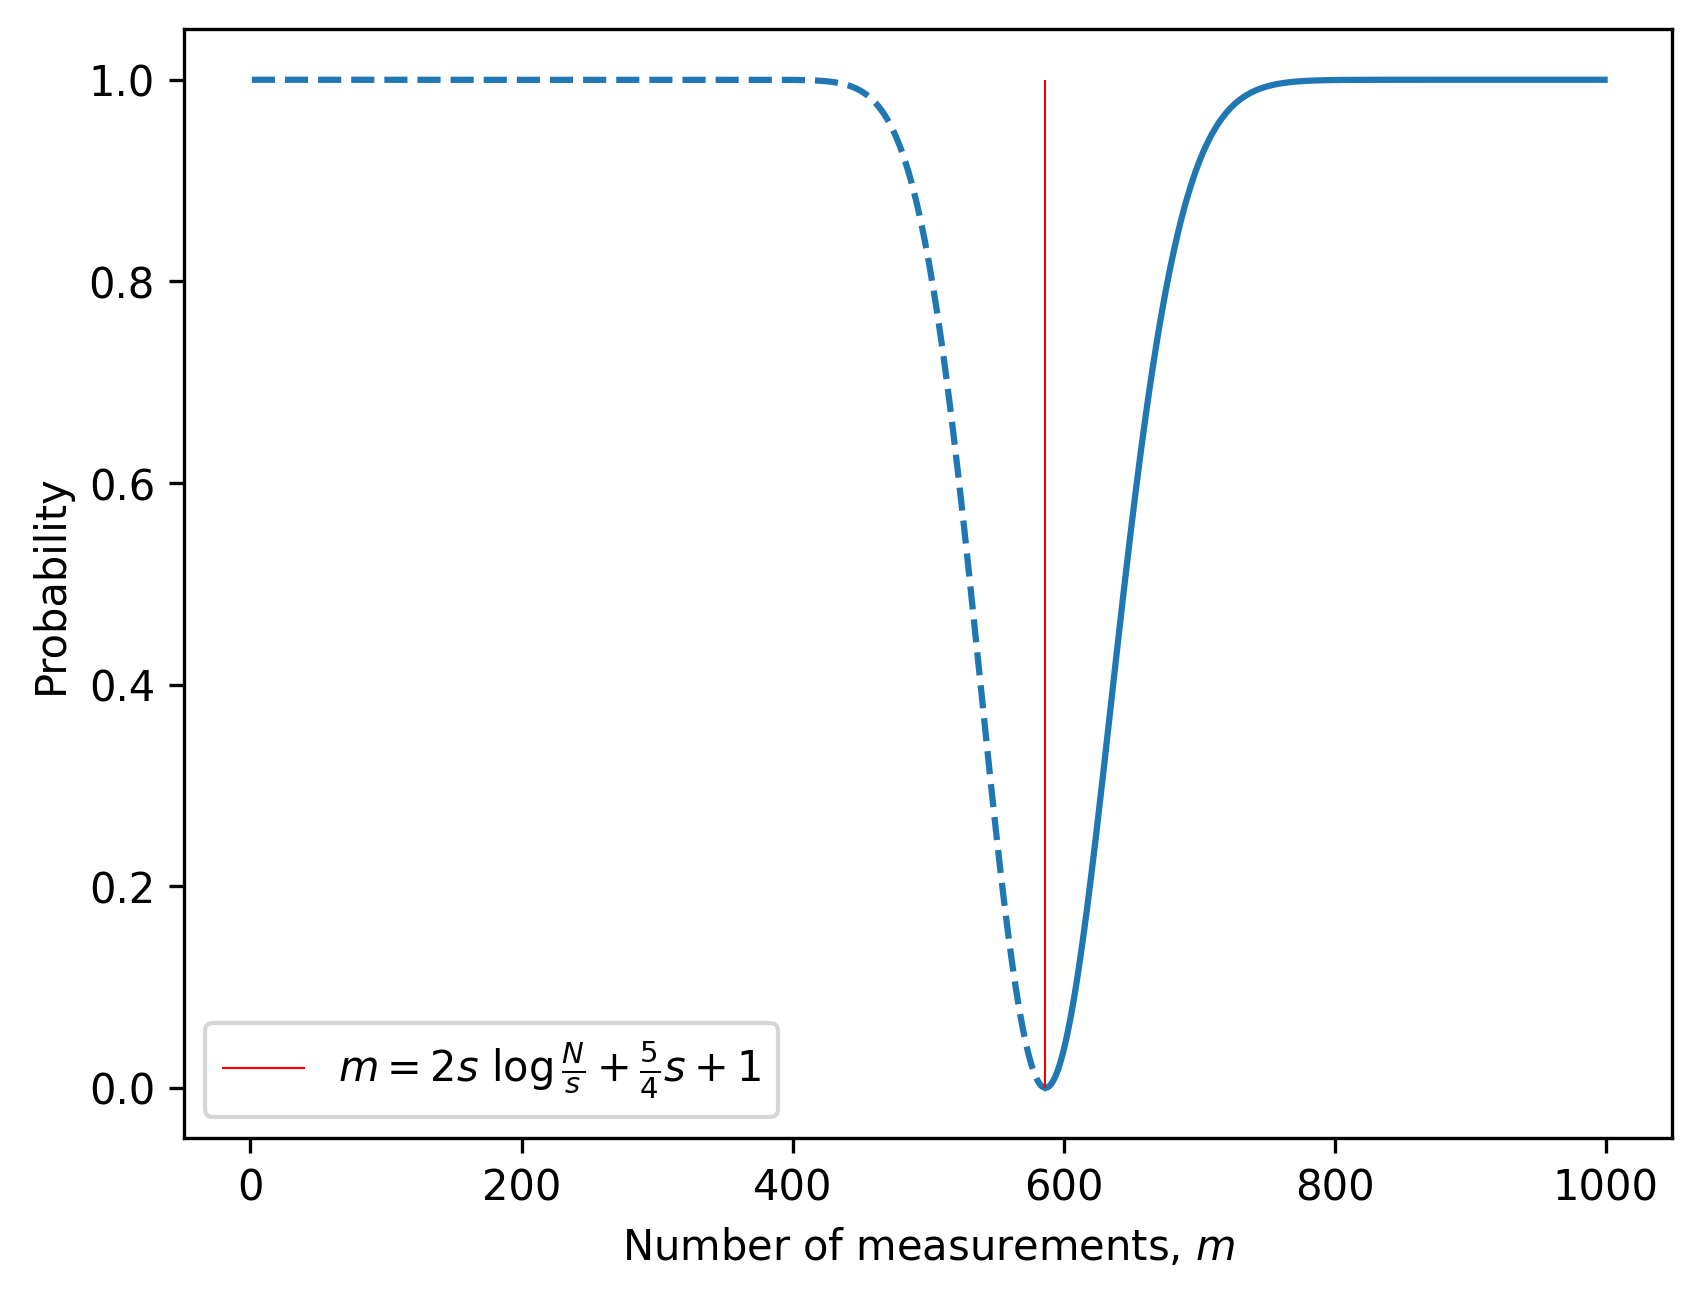
\includegraphics[width=\linewidth]{pictures/log_proba1000}
        \caption{}
    \end{subfigure}
    \caption{\centering Plots for the probability estimate as seen in (\ref{eq:log_improved}).
    In (a) $N=100$, $s=10$, while in (b) $N=1000$, $s=100$.}
    \label{fig:log-proba}
\end{figure}

\begin{remark}
    In the paper, authors formulate this result without specifying the probability and just referring to it as being ``high''.
    And it is, no doubt, high; however, we can try studying that in more detail.
    At this point, the expression for probability contains $w(\Omega)$, which is not great for numerical experiments.
    According to Theorem~\ref{th:yibucha}, ``success'' requires $m \geq w(\Omega)^2+1$.
    This gives us our first inequality, $w(\Omega) \leq \sqrt{m-1}$.
    As for the $\lambda_m$, it can be proven that $\frac{m}{\sqrt{m+1}} \leq \lambda_m \leq \sqrt{m}$.
    By combining that we get \[\lambda_m - w(\Omega) \geq \frac{m}{\sqrt{m+1}} - \sqrt {m-1} \geq 0.\]
    The function $f(x) = 1 - \exp\left(-\frac{1}{2}(\lambda-x)^2\right)$ is monotonically decreasing for $x \leq \lambda$.
    To use this fact and combine it with the estimate for $w(\Omega)$, we first have to verify that $\frac{m}{\sqrt{m+1}} \geq \sqrt {2s \log \frac{N}{s} + \frac{5}{4}s}$
    or, equivalently, $\frac{m^2}{m+1} \geq 2s \log \frac{N}{s} + \frac{5}{4}s$.
    Let us denote $\alpha = 2s \log \frac{N}{s} + \frac{5}{4}s$.
    If we use the fact $m \geq \alpha$ and monotonicity of $\frac{m^2}{m+1}$ for $m \geq 0$, we get
    \[ \frac{m^2}{m+1} - a \geq \frac{(a+1)^2}{a+2} - a = \frac{1}{a+2} > 0,\]
    which allows us to conclude that
    \begin{align}
         m \geq 2s\log \frac{N}{s} + \frac{5}{4}s + 1 \implies &\mathbb{P}\{\x^* \text{ is the unique solution of \ref{eq:l1}}\} \nonumber \\
    & \geq 1 - \exp \left( - \frac{1}{2} \left[\frac{m}{\sqrt{m+1}} - \sqrt {2s \log \frac{N}{s}+\frac{5}{4}s}\right]^2 \right) \label{eq:log_improved}.
    \end{align}

    This is a more practical result, suitable for numerical study.
    The curves for probability from the last inequality is depicted in Fig.~\ref{fig:log-proba}.
    Note, that the only relevant information on those plots lies to the right of the red line, as in the derivation of this
    result we assumed that $m > 2s \log \frac{N}{s} + \frac{5}{4}s + 1$.
    From these plots we see that we can speak of ``high'' probability only if the ambient dimension is large enough.
\end{remark}

\subsection{Statistical dimension approach}

\begin{figure}
    \begin{subfigure}{0.5\textwidth}
            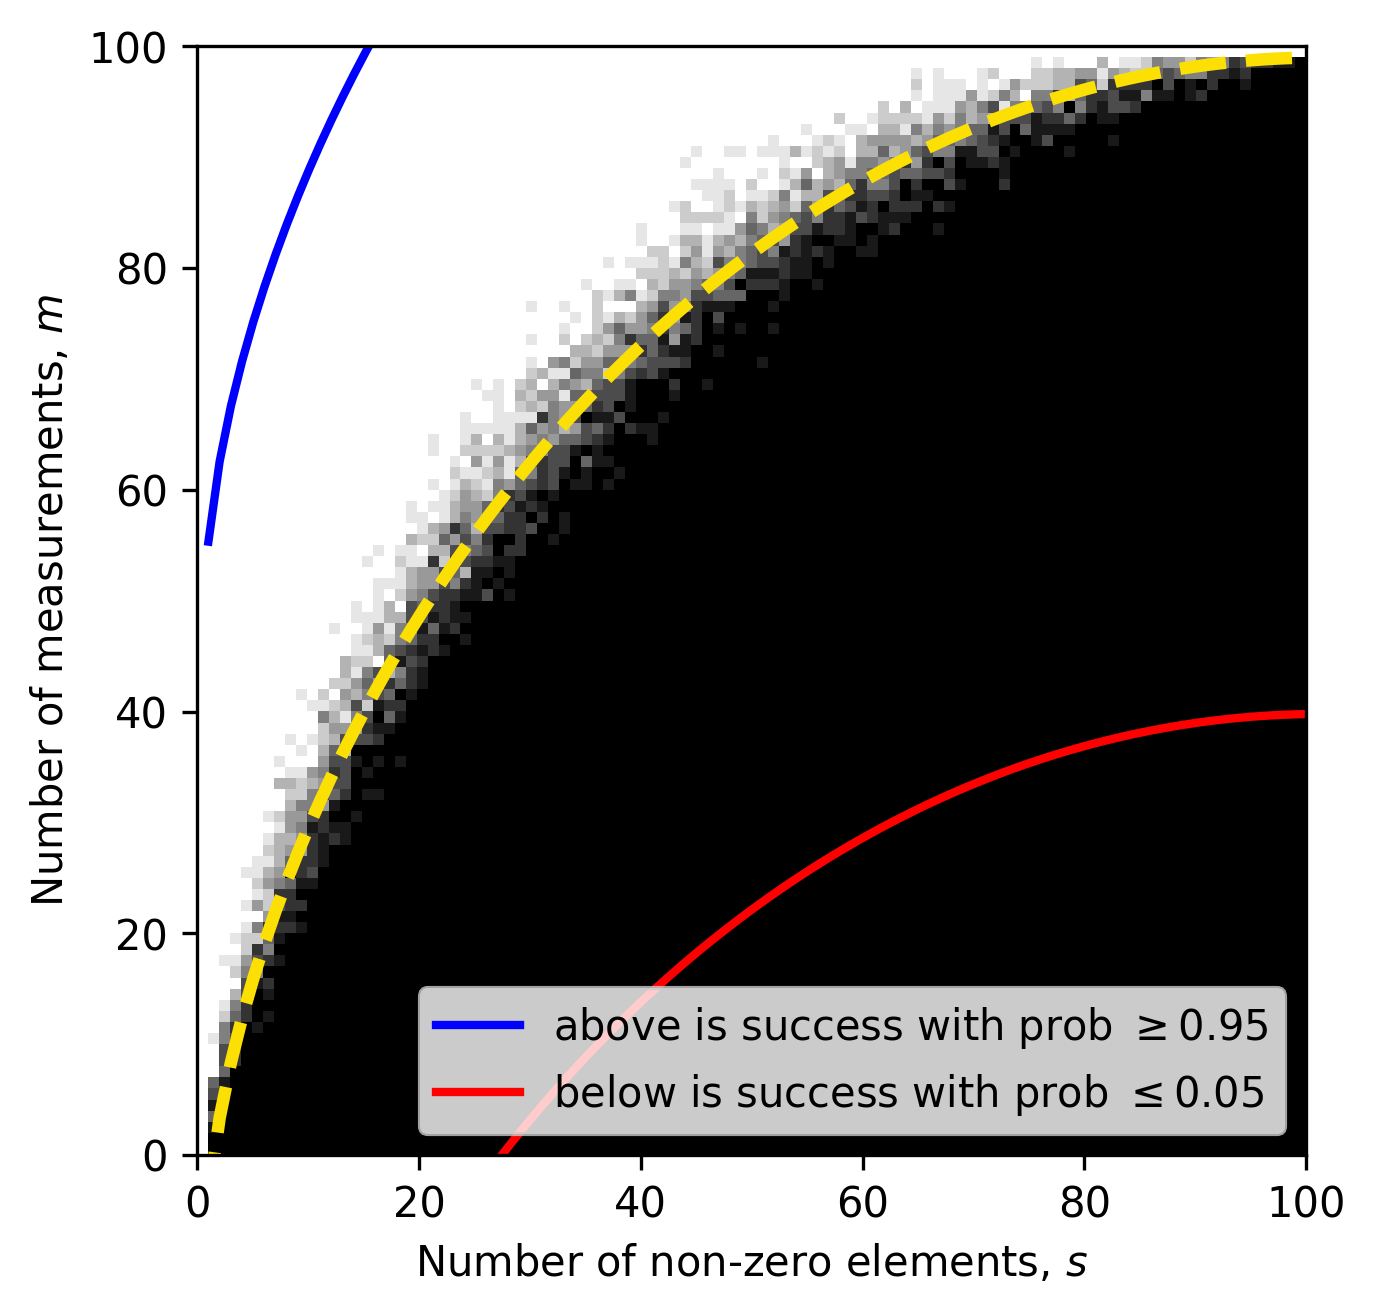
\includegraphics[width=\linewidth]{pictures/lote_estimates}
        \caption{}
    \end{subfigure}
    \begin{subfigure}{0.5\textwidth}
            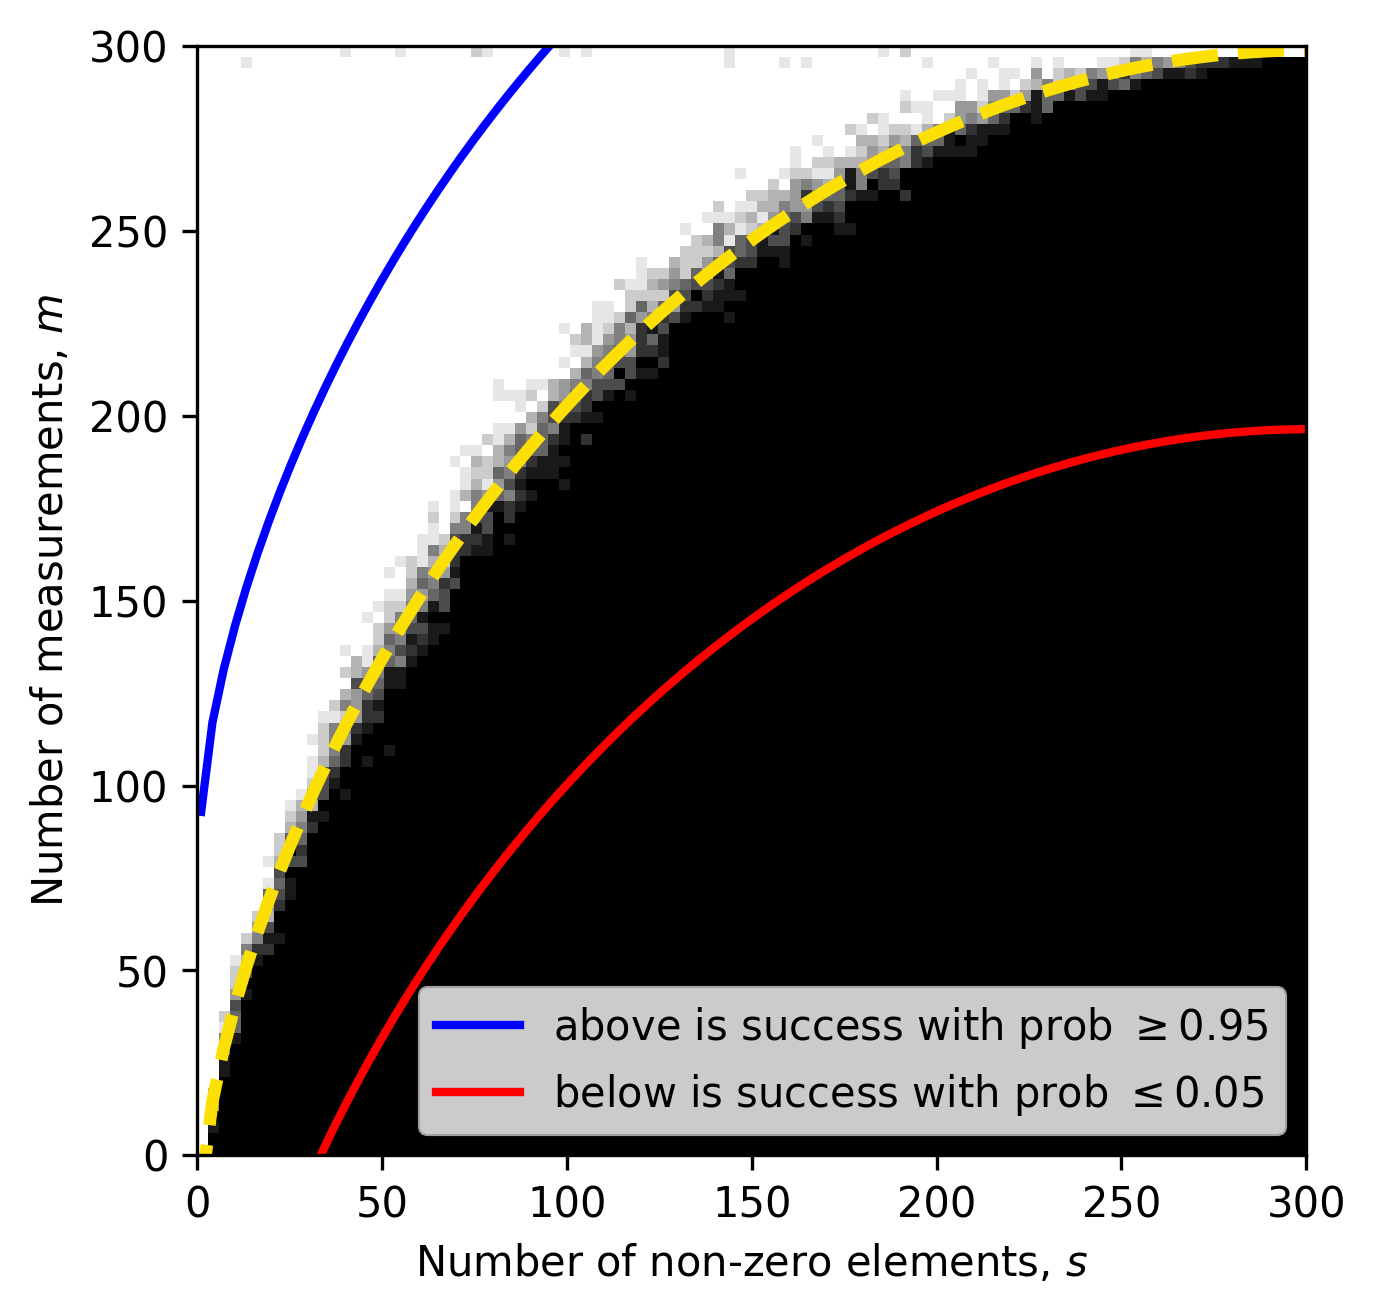
\includegraphics[width=\linewidth]{pictures/lote_estimates_d300}
        \caption{}
    \end{subfigure}

    \caption{Living on the Edge}
    \label{fig:lote}
\end{figure}

Another way to ``measure'' a cone for our purpose is proposed in~\cite{livingontheedge}.
Authors of the paper look at the result of the Proposition~\ref{th:dcker} in the context of conic integral geometry
and connect it with another problem: ``What is the probability of a randomly rotated convex cone to intersect a fixed convex cone?''.
It was known before that this problem is answered by the kinematic formula for cones, which relies on the notion of conic intrinsic volumes.
We will not dive into details of intrinsic volumes, but instead look at one simple example: polyhedral cones.
It is much easier to interpret and describes the intuition behind this concept.

As usual, we first list some definitions from convex geometry as given by~\cite{rockafellar}.
We will denote by $[\x, \y]$ the line segment connecting points $\x$ and $\y$, i.e., the set $\{{t\x + (1-t)\y,} \\ {t \in [0, 1]} \}$.

\begin{definition}
    The \textit{relative interior} $\op{ri} C$ of a convex set $C \subset \mathbb{R}^N$ is defined as
    \[ \op{ri} C = \{ \x \in \op{aff} C: \exists \varepsilon>0, B(\x, \varepsilon) \cap \op{aff} C \subset C \},\]
    where $\op{aff} C$ is the affine hull of the set $C$, i.e.,\ the smallest affine space that contains $C$,
    and $B(\x, \varepsilon)$ is the ball of radius $\varepsilon$ centered in $\x$.
\end{definition}

\begin{definition}
    Let $C' \subset C \subset \mathbb{R}^N$ be convex sets.
    If for every $\x, \y \in C$, such that $\op{ri}~[\x, \y ] \cap C' \neq \emptyset$, both $x$ and $y$ are in $C'$,
    then $C'$ is called a \textit{face} of $C$.
\end{definition}

\begin{definition}
    Let $\mathcal{C} \subset \mathbb{R}^N$ be a polyhedral cone.
    For $k \in [\![ 1..N ]\!]$, the $k$th \textit{conic intrinsic volume} is defined as
    \[ \nu_k(\mathcal{C}) = \mathbb{P} \left\{ \op{proj_\mathcal{C}} \mathbf{g} \text{ lies in the relative interior
    of a $k$-dimensional face of $\mathbb{C}$} \right\}, \]
    where $\mathbf{g} \sim \mathcal{N}(\mathbf{0}, \mathbf{I})$ is a vector of independent random variables with standard normal distribution.
\end{definition}

\contourlength{1.5pt}
\begin{figure}
    \begin{subfigure}{0.48\linewidth}
        \centering
        \begin{tikzpicture}
            \path[fill=teal, fill opacity=0.15] (0,0) -- (-4, 2.5) -- (-4, -2.5) -- (0,0) --cycle;
            \begin{scope}
                \clip (0,0) -- (-4, 2.5) -- (-4, -2.5) -- (0,0) --cycle;
                \node[circle,draw=,minimum size=30pt] at (0,0) (circ) {};
            \end{scope}
            \node at (-0.5, 0) [left]{$\phi$};
            \filldraw (-0.5, 2) circle (1pt);
            \draw[dashed] (-0.5, 2) -- (-1.27, 0.77)
            \node at (-0.5, 2) [right]{$\mathbf{g}$}
            \draw[teal, line width=1pt] (0,0) -- (-4, 2.5);
            \draw[teal, line width=1pt] (0,0) -- (-4, -2.5);
            \draw (0,0) -- (1.56, 2.5);
            \draw (0,0) -- (1.56, -2.5);
            \filldraw (-1.26, 0.79) circle (1pt);
            \node at (-1.26, 0.79) [below=5pt, left]{$\op{proj}_\mathcal{C}\mathbf{g}$};
            \path[pattern=dots] (0,0) -- (1.56, 2.5) to[curve through={(2.5, 0)}] (1.56, -2.5) -- (0,0) --cycle;
            \begin{scope}
                \clip (0,0) -- (1.56, 2.5) to[curve through={(2.5, 0)}] (1.56, -2.5) -- (0,0) --cycle;
                \node[circle,draw=,minimum size=30pt] at (0,0) (circ) {};
                \node[circle,draw=,minimum size=26pt] at (0,0) (circ) {};
            \end{scope}
            \node at (0.5, 0) [right]{\contour{white}{$\pi-\phi$}};
            \node at (-3.5, -1.25) {$\mathcal{C}$};
            \node at (1.7, -1.25) {\contour{white}{$\mathcal{C}^*$}};
            \filldraw[teal] (0, 0) circle (2pt);
        \end{tikzpicture}
        \caption{}
        \label{fig:cones_a}
    \end{subfigure}
    \hfill
    \begin{subfigure}{0.48\linewidth}
        \centering
        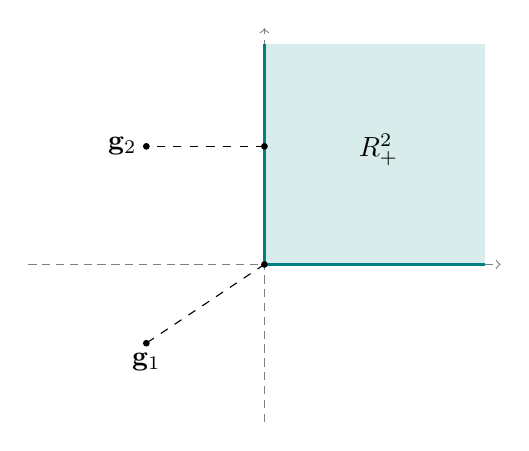
\begin{tikzpicture}
            \draw[densely dashed, gray][->] (0, -2) -- (0, 3);
            \draw[densely dashed, gray][->] (-3, 0) -- (3, 0);
            \path[fill=teal, fill opacity = 0.15] (0, 0) -- (0, 2.8) -- (2.8, 2.8) -- (2.8, 0) -- (0, 0) -- cycle;
            \draw[teal, line width=1pt] (0, 0) -- (0, 2.8);
            \draw[teal, line width=1pt] (0, 0) -- (2.8, 0);
            \filldraw (0, 0) circle (1pt);

            \begin{scope}
                \filldraw (-1.5, -1) circle (1pt);
                \draw[dashed] (0, 0) -- (-1.5, -1);
                \node at (-1.5, -1) [below]{$\mathbf{g}_1$};
            \end{scope}
            \begin{scope}
                \filldraw (-1.5, 1.5) circle (1pt);
                \filldraw (0, 1.5) circle (1pt);
                \draw[dashed] (0, 1.5) -- (-1.5, 1.5);
                \node at (-1.5, 1.5) [left]{$\mathbf{g}_2$};
            \end{scope}
            \node at (1.45, 1.45) {$\mathbb{R}^2_+$};
        \end{tikzpicture}
        \caption{}
    \end{subfigure}
    \caption{cone}
    \label{fig:cones}
\end{figure}

For an arbitrary cone, we first approximate it with polyhedral cones and then define the $k$th intrinsic volume as the limit
of the sequence formed by $k$th intrinsic volumes of the approximating sequence.

\begin{definition}
    Let $\mathcal{C} \subset \mathbb{R}^N$ be a closed convex cone.
    The statistical dimension $\delta (\mathcal{C})$ of the cone $\mathcal{C}$ is then defined as
    \[\delta(\mathcal{C}) = \sum_{k=0}^N k \nu_k (\mathcal{C}).\]
\end{definition}

\begin{example}
    Let $\mathcal{C} \subset \mathbb{R}^2 $ be a convex cone as shown in Fig.~\ref{fig:cones_a}.
    It has one zero-dimensional face (\{$\mathbf{0}$\}, the origin point), two one-dimensional faces (the two boundary rays)
    and one two-dimensional face (the cone itself).
    For the projection of vector $\mathbf{g}$ to be in the relative interior of a zero-dimensional face (which is also $\{\mathbf{0}\}$),
    the vector $\mathbf{g}$ has to be inside of the polar of $\mathcal{C}$, i.e., $\mathbf{g} \in \mathcal{C}^*$.
    The standard normal distribution is rotationally symmetric, so $\mathbb{P}\{ \mathbf{g} \in \mathcal{C}^*\} = \frac{\pi - \phi}{2\pi} $.
    Similarly, for $\op{proj}_{\mathca{C}} \mathbf{g}$ to lie inside $\mathcal{C}$, $\mathbf{g}$ itself must be inside of $\mathcal{C}$,
    which happens with probability $\frac{\phi}{2\pi}$.
    Finally, for one-dimensional faces we have the probability $\frac{1}{2}$.
    The statistical dimension can be easily calculated from the definition as
    \[ \delta (\mathcal{C}) = \frac{1}{2} + 2\frac{\phi}{2\pi} = \frac{\pi + 2\phi}{2\pi}.\]
\end{example}

\begin{example}
    The non-negative orthant $\mathbb{R}^N_+$ forms a polyhedral cone as an intersection of two half-spaces.
    It has one zero-dimensional face $\{\mathbf{0}\}$, $N$ one-dimensional faces of the form $\{0\}^k \times \mathbb{R}_+ \times \{0\}^{N-k-1}$
    for $k \in [\![ 0..N-1 ]\!]$, $\frac{N(N-1)}{2}$ two-dimensional faces of the form
    $\{0\}^k \times \mathbb{R}_+ \times \{0\}^j \times \mathbb{R}_+ \times \{0\}^{N-k-j-2}$ for
    $(k, j) \in  [\![ 0..N-2 ]\!]^2$ with $k+j = N-2$ and so on.
    In other words, $k$-dimensional faces only contain vectors with exactly $k$ non-zero components.
    Then $\op{proj}_{\mathbb{R}^N_+} \mathbf{g}$ lies in the relative interior of a $k$-dimensional face of $\mathbb{R}^N_+$
    if and only if $\mathbf{g}$ has exactly $k$ positive components, so
    \begin{equation*}
        {\nu_k(\mathbb{R}^N_+) = \mathbb{P}\{ \mathbf{g} \text{ has exactly } k \text{ positive components} \} }.
    \end{equation*}
    There are $\binom{N}{k}$ ways to ``choose'' which components will be positive.
    The probability of each component to be positive is $1/2$; the probability of it to be negative is also $1/2$.
    As they are independent from each other, we get the result
    \[{\nu_k(\mathbb{R}^N_+) = \frac{1}{2^N} \binom{N}{k}. \]
    The statistical dimension is then
    \[\delta (\mathbb{R}^N_+) = \frac{1}{2^N}\sum_{k=0}^N k \binom{N}{k} = \frac{N}{2^N} \sum_{k=0}^{N-1} \binom{N-1}{k} = \frac{N}{2}.\]
\end{example}

The topic of statistical dimension and conic intrinsic volumes is discussed in more detail in~\cite{statdim}.

\begin{theorem}
    Let $\x^* \in \mathbb{R}^N$ be a fixed vector and $p \in (0, 1)$.
    Suppose $\A \in M_{m \times N}(\mathbb{R})$ is a matrix with independent $\mathcal{N}(0,1)$-distributed entries and
    $\y = \A \x^*$.
    Then
    \begin{align*}
        & m \leq \delta(\mathcal{D}(\norm{\cdot}_1, \x^*)) - a_\eta \sqrt{N} \implies
        \mathbb{P}\{\x^* \text{ is the unique solution of \ref{eq:l1}}\} \leq \eta
        \\
        & m \geq \delta(\mathcal{D}(\norm{\cdot}_1, \x^*)) + a_\eta \sqrt{N} \implies
        \mathbb{P}\{\x^* \text{ is the unique solution of \ref{eq:l1}}\} \geq 1 - \eta,
    \end{align*}
    where $a_\eta = \sqrt{8 \log (4/\eta)}$.
    \label{th:lote}
\end{theorem}

\begin{figure}
    \begin{subfigure}{0.5\textwidth}
        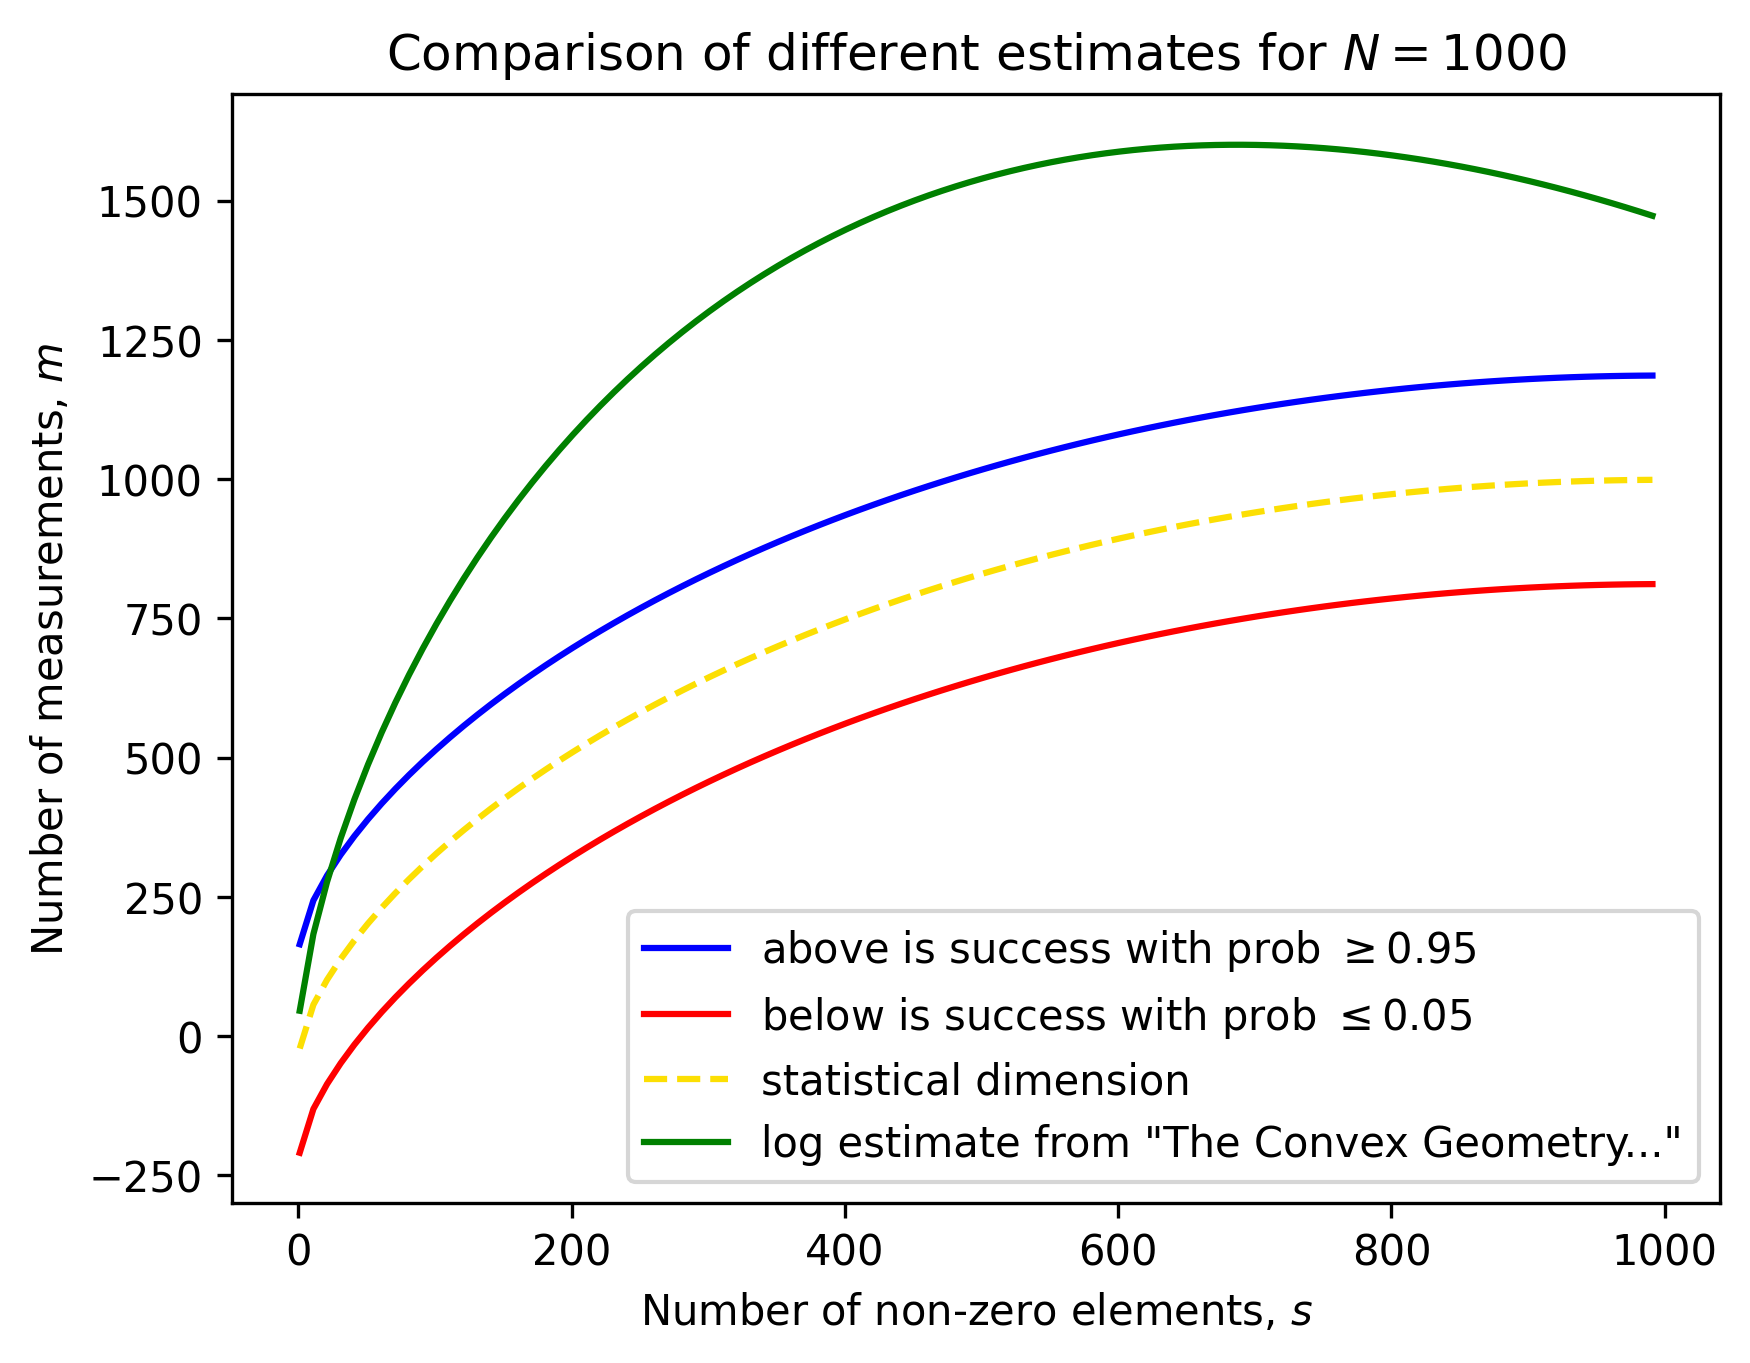
\includegraphics[width=\linewidth]{pictures/compare_estimates1000}
    \end{subfigure}
    \begin{subfigure}{0.5\textwidth}
        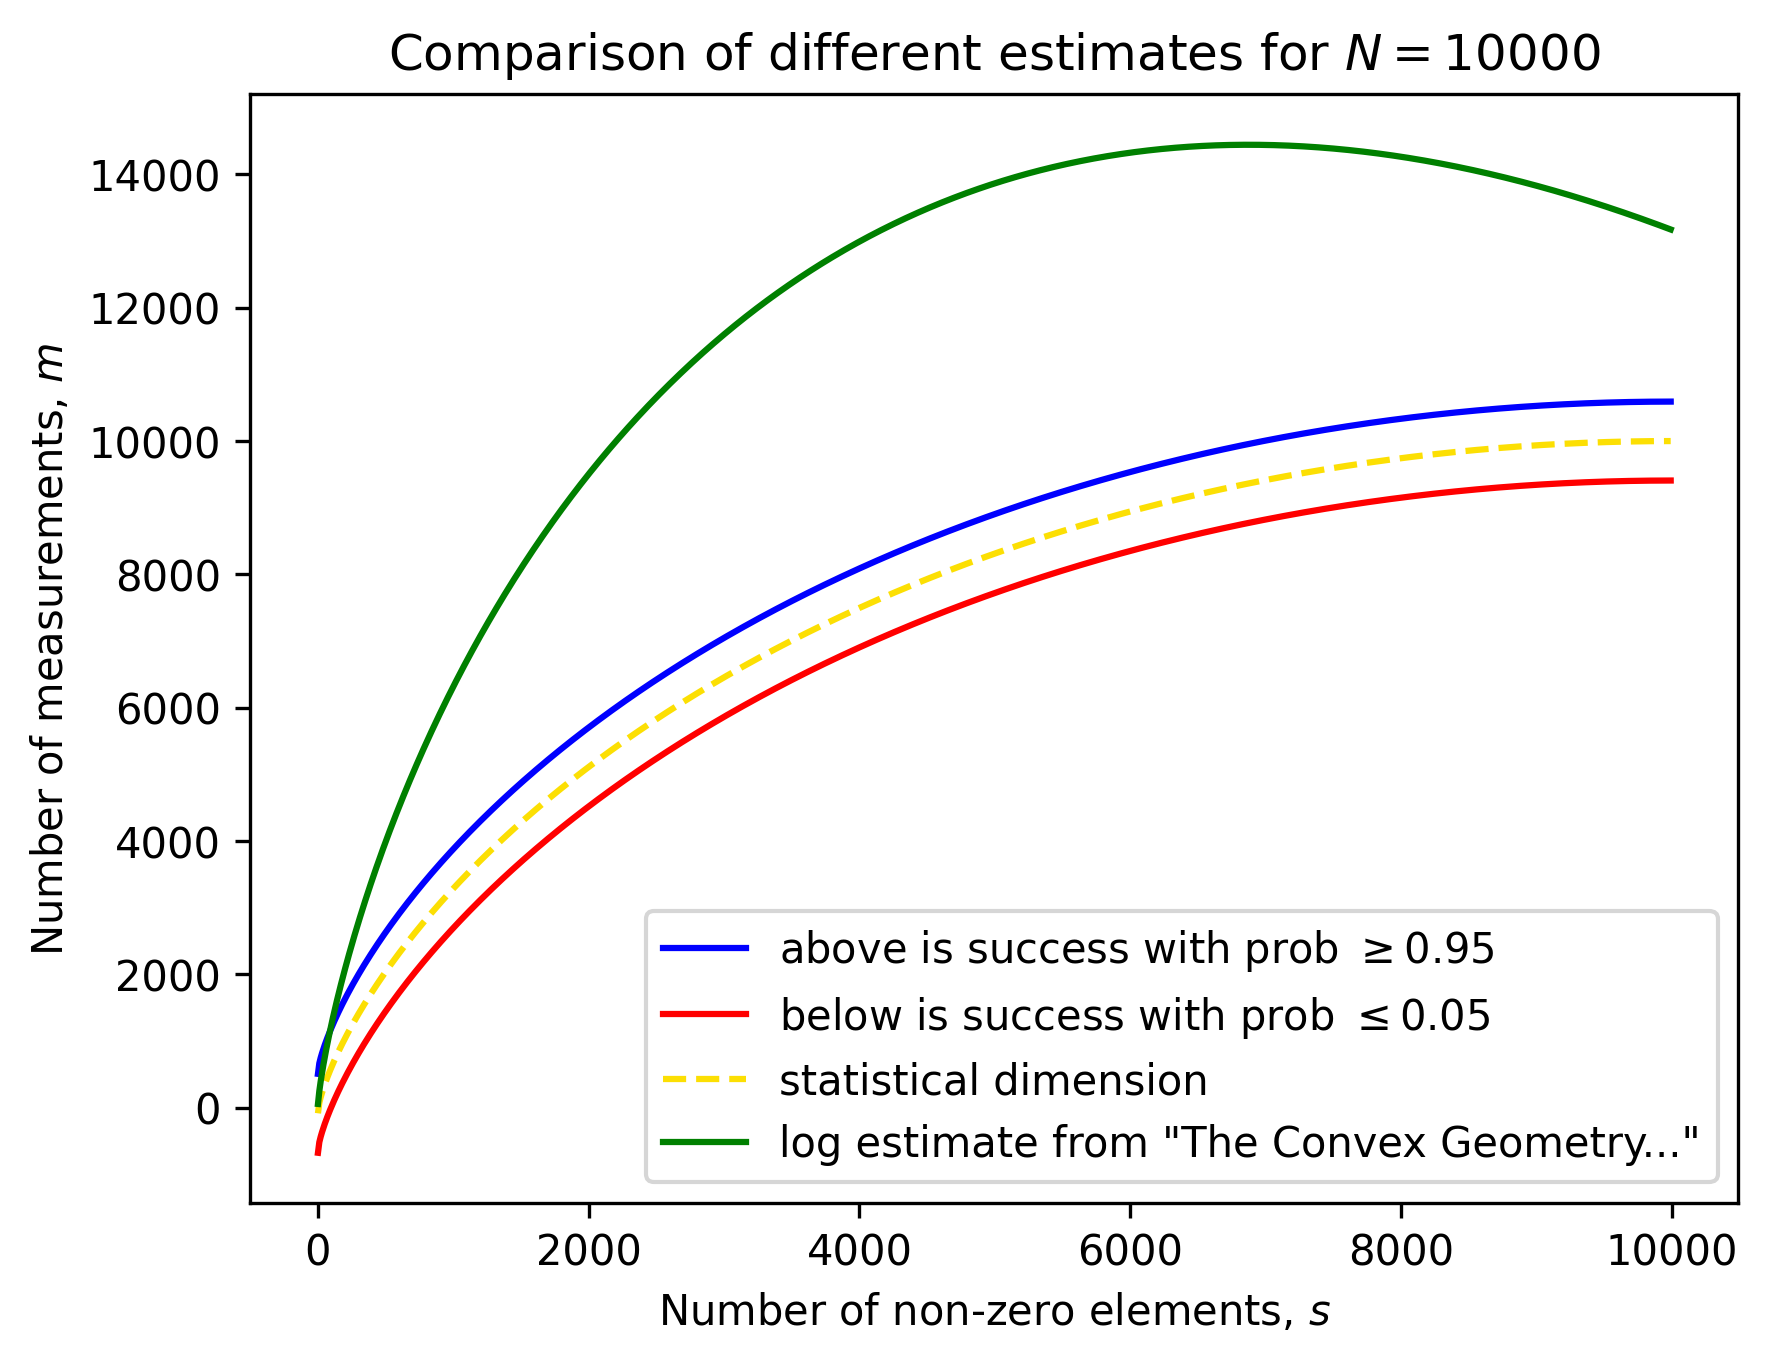
\includegraphics[width=\linewidth]{pictures/compare_estimates10000}
    \end{subfigure}
    \caption{Comparison}
    \label{fig:compare}
\end{figure}